\begin{frame}
    \begin{center}
        \begin{tikzpicture}
            \node[anchor=south west,inner sep=0] (image) at (0,0) {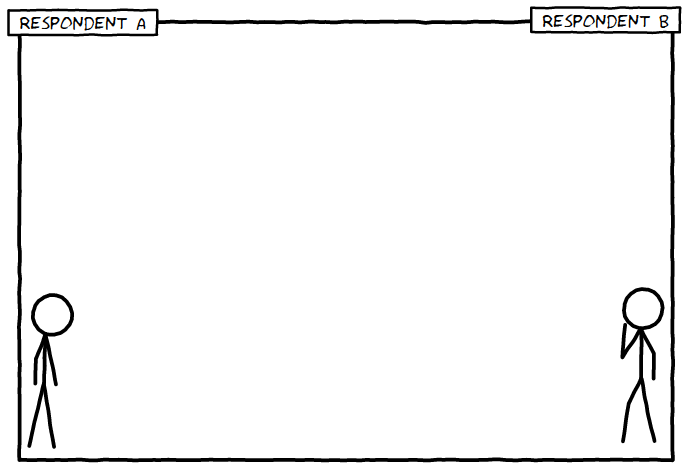
\includegraphics[width=.9\textwidth]{fig/Respondents_empty.png}};
            \node[align=center] at (image.center) {\Large \emph{Conclusion}};
        \end{tikzpicture}
    \end{center}
\end{frame}


\subsection{General Discussion}

\begin{frame}%[allowframebreaks]
  \frametitle{General Discussion}
  \begin{itemize}
\item We observe \emph{theoretically meaningful} variation in the \emph{complexity} of verbatim open-ended responses.
%\item Discursive sophistication and conventional knowledge measures \emph{share a substantial amount of variance}, but they are far from identical.
\item<2->  By directly examining how individuals \emph{justify their attitudes}, we can measure sophistication related to \emph{specific political tasks}.
\item<3-> Discursive sophistication is conceptually closer to the \emph{structure of belief systems} than conventional measures.

\vspace{1em}
\item<4-> Women might score lower than men on \emph{factual knowledge} about political institutions, but there are no differences in the \emph{sophistication} of expressed political attitudes.
%\begin{center}\emph{\texttt{\#WomenAlsoKnowStuff}}\end{center}
\end{itemize}
\end{frame}
%Information vs. competence argument by Lupia!!


\begin{frame}{Illustration -- Who scores higher on political knowledge?}
    \begin{center}
        \begin{tikzpicture}
            \node[anchor=south west,inner sep=0] (image) at (0,0) {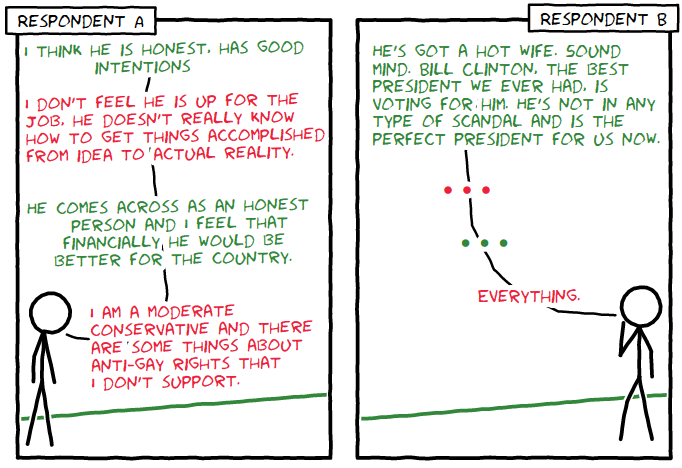
\includegraphics[width=.9\textwidth]{fig/Respondents8.png}};
            \node<2->[anchor=south west,inner sep=0] (image) at (1.4,2) {
\includegraphics[width=.3\textwidth]{fig/We_Can_Do_It!.jpg}};
            \node<3->[anchor=south west,inner sep=0] (image) at (5.8,3.5) {
\includegraphics[width=.3\textwidth]{fig/skinny-man.jpg}};
        \end{tikzpicture}
    \end{center}
\end{frame}


\begin{frame}%[allowframebreaks]
  \begin{center}
  \large{Thank you very much for your attention!}\\ \vspace{2em}
  Manuscript and code available at:\\
  %\emph{\texttt{https://github.com/pwkraft/mft}}\\
  \emph{\texttt{https://github.com/pwkraft/knowledge}}\\ \vspace{2em}
  Comments, questions?\\
  \emph{\faEnvelopeO\hspace{.5em}\texttt{kraftp@uwm.edu}}\\\vspace{2em}
  \emph{\faGlobe\hspace{.5em}\texttt{pwkraft.github.io}}\\
  \emph{\faTwitter\hspace{.5em}\texttt{@patrickwkraft}}\\
  \end{center}
\end{frame}

% RESPONSE to question about rationalization:
% I think that is a fair point and that is something that we definitely have to take into account when interpreting these results. But I would think of it as not being a bug but rather a feature of the approach. In Druckman's 2014 article on the "Pathologies of Studying Public Opinion", he makes the argument that it is unclear whether factual information is necessary for people to have quality opinions. Instead, he argues that we should look at the process by which people come to their opinions, and what he means is whether people are motivated to come to an accurate opinion. In psychology, accuracy motivation is often induced by asking people to justify their opinions. So I think it makes sense to examine how well they are sophisticated in providing these justifications in order to assess whether their opinions are indeed well-grounded and based on careful consideration.